\subsection{Introduction}
\par
In this research we try to define and solve a realistic and complete problem that considers the placement problem besides the management resources.
In our problem we consider many requirements including:

\begin{itemize}
    \item Some of the physical servers may not be managed by specific set of physical server because of their distance or security concerns.
    \item VNFs have typs and may be there are restrictions on their placement.
    \item Each VNFM needs a license for managing the specific number of VNF instances.
    \item Each VNFM can manage VNFs that have hop count less than specific number.
\end{itemize}

\subsection{Problem}
\par
Infrastructure topology is know as a directed graph \(G(V, E)\). \(V\) is a set of NVFI-PoPs with RAM and CPUs and \(E\) is a set of links with bandwidth.
Some nodes of \(V\) are ingress and egress nodes so chains must start and end in those node accordingly. Some of the infrastructure nodes cannot handle VNFs.
\(n\) chains' request known apriori with their specifications and requirements. Each request VNFs' type are know besides their links' bandwidth.
There are \(F\) VNFs' types and each type has its specific memory and processing requirement.
We consider memory and cpu resource constraints on each node for its VNFs and VNFMs.
Each VNFM needs license and can handle specific number of VNFs.
For having a better delay in management links, we reserve bandwidth between VNFs and VNFMs and also there is an specific radius that VNFMs can manage VNFs.
We don't share VNFs between chains and each chain has a single VNFM for consistent management and monitoring but we share VNFMs between chains.
As we mentioned, some of the physical servers may not be managed by specific set of physical server because of their distance or security concerns.
We want to place chains with their VNFM to maximize profit. Accepting each chain has specific gain and buying license costs.

\subsection{Example}
\par
Here we want to consider an illustrative example to gain more sight into described problem.
Figure~\ref{fig:example-chains} shows request chains with their type and links. link required bandwidth are Mbps.
We try to place these chains into Figure~\ref{fig:example-topology}.
VNFs' type are described in Table~\ref{tbl:example-vnf-types}.
Table~\ref{tbl:example-server-spec} describes the physical servers specifications.
Instances can only run on servers 1, 3, 5, and 7.
Servers 1 and 3 can only be managed by the servers 2 and 4.
Server 5 can only be managed by the servers 4 and 6.
Server 7 can only be managed by the servers 6 and 8.
Each VNFM can handles 5 instances with 4 GB of RAM and 2 CPU cores.
All physical links has 40Gbps capacity.

\begin{figure}
    \centering
    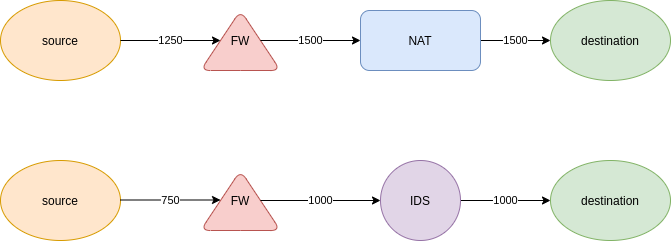
\includegraphics[height=150px]{images/example-chains.png}
    \caption{Chains for illustrative example}
    \label{fig:example-chains}
\end{figure}

\begin{figure}
    \centering
    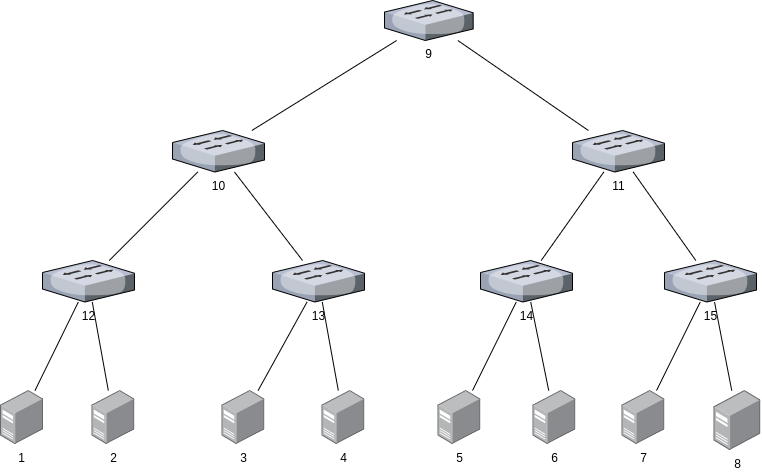
\includegraphics[height=150px]{images/example-toplogy.png}
    \caption{Topology of illustrative example}
    \label{fig:example-topology}
\end{figure}

\begin{table}
    \centering
    \caption{VNFs type of illustrative example}
    \begin{tabular}{|c|c|c|c|}
        \hline
        Spec/VNF & vFW & vNAT & vIDS \\
        \hline
        CPU (vCore) & 2 & 2 & 2 \\
        \hline
        Memory (GB) & 2 & 4 & 2 \\
        \hline
    \end{tabular}
    \label{tbl:example-vnf-types}
\end{table}

\begin{table}
    \centering
    \caption{Server specification of illustrative example}
    \begin{tabular}{|c|c|c|}
        \hline
        & Server 1,2,7,8 & Servers 3,4,5,6 \\
        \hline
        Installed vCPU & 144 & 72 \\
        \hline
        Installed Memory (GB) & 1408 & 288 \\
        \hline
        Link (Gbps) & 40 & 40 \\
        \hline
    \end{tabular}
    \label{tbl:example-server-spec}
\end{table}

\subsection{Importance}
\par
This problem considers VNFs and their requirements for management by a VNFMs. Considerations in this problem tries to be realistic and be useful at data centers.